\problemname{Fredriks pizzeria}
\noindent

Din kompis Elsa jobbar som en nattvakt i Fredriks pizzeria.
I pizzerian finns det $N$ stycken rum och $M$ stycken oriktade korridorer, numrerade från $1$ till $N$ och $1$ till $M$ respektive.
Hon befinner sig just nu i rum $1$.
Nattskiftet tog precis slut, och hon vill ta sig hem genom utgången i rum $2$.
Tyvärr finns det en ondskefull råtta som befinner sig i rum $3$ som försöker stoppa henne.
För att skydda sig från denna har varje korridor en elektronisk dörr som hon kan stänga.
Varken Elsa eller råttan kan passera igenom en stängd dörr.
Hon kan öppna och stänga dörrar hur hon vill, med ett krav:
varje dörr är sammanlänkad med exakt en annan dörr.
Om två dörrar är sammanlänkade innebär det att om den ena är stängd måste den andra vara stängd.
På samma vis, om den ena är öppen måste den andra vara öppen.
En viss dörr kan inte vara sammanlänkad till mer än en annan dörr.

Eftersom kontrollpanelen finns i hennes kontor i rum $1$, så måste hon bestämma vilka korridorer hon ska öppna innan hon lämnar kontoret.
När hon väl lämnat kontoret är hennes enda chans att ha stängt dörrar så råttan inte kan ta sig till henne genom korridorer med öppna dörrar, samtidigt som hon kan ta sig till utgången genom korridorer med öppna dörrar.
Även om hennes kontor skulle ligga bredvid utgången är råttan så snabb att hon inte skulle hinna ta sig ut i tid om råttan kunde nå henne.

Avgör om det finns ett sätt att stänga dörrar så att Elsa kan ta sig ut, samtidigt som råttan
inte kan nå henne.

På grund av brandsäkerhet är det även garanterat att varje korridor ingår i som mest en cykel\footnote{Definitionen av en cykel med $k$ ($k \geq 3$) rum är en sekvens rum $c_1, c_2, \dots, c_k$, där alla $c_i$ är parvis unika och det finns en korridor mellan $c_i$ och $c_{i+1}$. Notera att det även måste finnas en korridor mellan $c_k$ och $c_1$. I synnerhet är ett enstaka rum, eller ett par av rum sammankopplade med en korridor inte en cykel, då $k < 3$ i dessa fallen.}.

\section*{Indata}
Den första raden av indata innehåller heltalen $N$ och $M$ ($3 \leq N \leq 2 \cdot 10^5$, $2 \leq M \leq 2 \cdot 10^5$),
antalet rum och korridorer i pizzerian. Det är garanterat att $M$ är jämnt.

Den $i$:te av de följande $M$ raderna innehåller vardera heltalen $u$, $v$ och $l$ ($1 \leq u,v \leq N$, $u \neq v$, $1 \leq l \leq M$, $l \neq i$),
vilket betyder att det finns en korridor mellan rum $u$ och $v$, och att denna korridor är sammanlänkad med korridoren med nummer $l$.
Korridorerna ges i samma ordning som de är numrerade.
Det är garanterat att det finns som mest en korridor mellan varje par av rum.
Det är även garanterat att korridoren är sammanlänkad med en \textit{annan} korridor och att sammanlänkningen av korridorer är symmetrisk: korridor $l$ är sammanlänkad med korridor $i$.

Det är även garanterat att man kan nå alla rum från rum $1$ om alla dörrar är öppna, och att varje korridor ingår i som mest en cykel.

\section*{Utdata}
Skriv ut ''\texttt{Ja}'' om det går att stänga dörrar så att Elsa kan ta sig ut samtidigt som råttan inte kan nå henne, annars ''\texttt{Nej}''.

\section*{Poängsättning}
Din lösning kommer att testas på en mängd testfallsgrupper.
För att få poäng för en grupp så måste du klara alla testfall i gruppen.

\noindent
\begin{tabular}{| l | l | p{12cm} |}
  \hline
  \textbf{Grupp} & \textbf{Poäng} & \textbf{Gränser} \\ \hline
  $1$    & $5$        & $N, M \leq 100$ och det finns inga cykler. \\ \hline
  $2$    & $10$       & Det finns inga cykler. \\ \hline
  $3$    & $12$       & $N, M \leq 100$ \\ \hline
  $4$    & $8$        & $N, M \leq 2000$ och varje rum ingår i som mest en cykel. \\ \hline % Vertex cactus
  $5$    & $15$       & $N, M \leq 2000$ \\ \hline
  $6$    & $19$       & Varje rum ingår i som mest en cykel. \\ \hline
  $7$    & $31$       & Inga ytterligare begränsningar. \\ \hline % edge cactus
\end{tabular}

\section*{Förklaring av exempelfall}
Alla exempelfall kommer att visualiseras på följande vis:
rum $1$ (startrummet) kommer att markeras grönt,
rum $2$ (utgången) blå,
och rum $3$ (råttans rum) rött.
Korridorerna kommer färgläggas så att korridorer med samma färg är sammanlänkade.

I exempelfall $1$ går det inte eftersom de enda korridorerna mellan utgången och råttan är sammankopplade.
Om Elsa väljer att öppna korridor $1$ och $2$ kommer råttan att stoppa henne.
Om hon stänger korridorerna kommer hon inte kunna komma ut.

\begin{figure}[h]
  \centering
  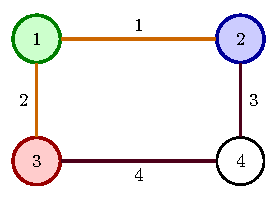
\includegraphics[width=0.4\textwidth]{sample1.pdf}
\end{figure}

I exempelfall $2$ går det.
En lösning är stänga paren av dörrar i korridorer $2,7$ och $4,5$.
Då kan råttan inte nå Elsa, samtidigt som hon kan ta sig ut genom att vandra igenom rummen $1,4,6,2$.
Detta fallet hade inte kunnat vara en del av grupp $4$ eller $6$ eftersom rum $6$ ingår
i två cykler (cyklerna $6,4,1,5$ och $6,7,3$).

\begin{figure}[h]
  \centering
  
\includegraphics[width=0.4\textwidth]{sample2.pdf}
\end{figure}
